\chapter{Introduction}\label{ch:Introduction}

% Overview
\section*{Overview}
This thesis introduces an entire compiler development for languages derived from LR(1) grammars. It involves:

\begin{itemize}
    \item Lexical analysis of both the source code and the input context-free grammar(CFG).
    \item Testing whether the input CFG is indeed LR(1).
    \item The source code pre-processing.
    \item Syntactic analysis, where the parser examines the refined token sequence to decode its hierarchical structure. The outcome is the parse tree, representing the complete hierarchical structure of the source code as per the input programming language's grammar.
    \item The thesis details the implementation of a data structure to store CFGs and the construction of a \({DK_{1}}\) automaton, as advised by Michael Sipser \cite{sipser}, to test the LR(1) status of the input grammar.
    \item The latter part of the thesis addresses the compiler backend, focusing on data structures for symbol tables and assembly generation from the provided derivation tree.
    \item At the end of the thesis you will see the compiled C0 codes.
\end{itemize}

% Focus
\section*{Focus}
Our study concentrates on the \(C0\) language, which merges \(C\)'s syntax with \(Free Pascal\)'s semantics. This language is defined using context-free grammar (CFG), as illustrated in \hyperref[fig:grammar_c0]{Figure 1.1}. We will test the language's ambiguity and then classify it according to LR(1) grammar. This will lead to the development of a detailed compiler, which we will implement using the \(Java\) programming language.

% Methodology and Implementation
\section*{Methodology and Implementation}
Our methodology and implementation are based on these books:
\begin{itemize}
    \item "System Architecture: An Ordinary Engineering Discipline" by Sabine Schmaltz, Petro Lutsyk, Wolfgang J. Paul. \cite{sysbook}
    \item "Introduction to the Theory of Computation"
    by Michael Sipser. \cite{sipser}
\end{itemize}
\setlength{\parindent}{0pt}

Leveraging this theoretical groundwork, we've designed an LR(1) context-free grammar tester and parser to process not just \(C0\) language, but also all other languages specified by CFGs, including \(C\), \(Java\), and the like.\\

The entire implementation in Java is accessible on \href{https://github.com/fyfsb/dcfg.git}{GitHub}.

\begin{itemize}
    \item The \hyperref[ch:Lexical and Syntactic Analysis]{Chapter 2} and all the corresponding code development is done by Toma Pirtskhelani.
    \item The \hyperref[ch:backend]{Chapter 3} and all the corresponding code development is done by Irakli Khotchava.
\end{itemize}

% C0 CFG
\begin{figure}[h!]
    \center
    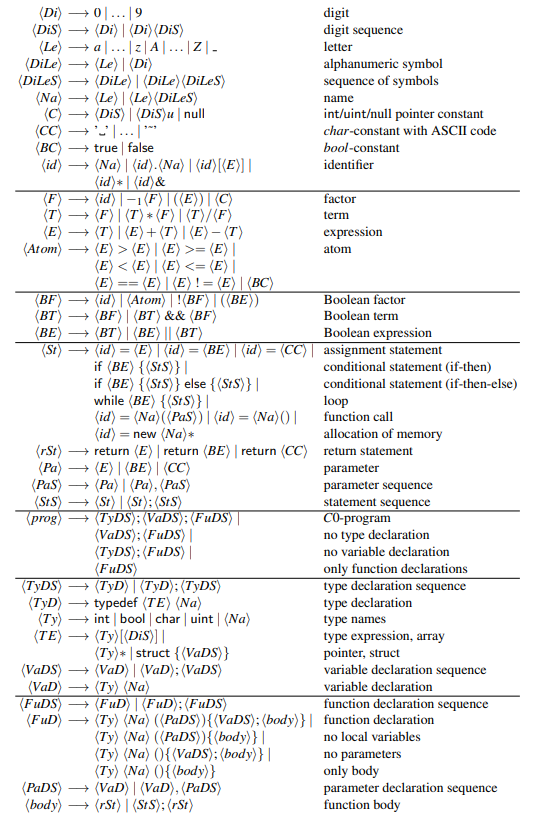
\includegraphics[width=13cm]{C0.png}
    \caption{C0 Context-Free Grammar}
    \label{fig:grammar_c0}
\end{figure}